\documentclass[salesmen, twoside]{../../../templates/latex/2009/softproj}
\usepackage[english]{babel} % For a load of tiny changes in the text
\usepackage{graphicx, ctable, url, hyperref} % graphics, tables, urls and cross-referencing

\usepackage{amsmath}
\usepackage{eurosym}

\title{Software Engineering Group 2 (2009-2010) \\Software Project Management Plan}
\author{Nick De Cooman}
\date {\today}

\begin{document}
\begin{projdoc}
	
	\chapter{Introduction}
	
		\section{Project overview}
		
			The goal of this project is to design and implement the software 
			behind an online auction website such as eBay. The codename of our project 
			is {\emph Salesmen}. The project is embedded in the Software Engineering course, 
			which is designed for senior students of Computer Science and Engineering 
			at the Vrije Universiteit Brussel. It has a threefold purpose:
			
			\begin{enumerate}
				\item Get familiar with the software development process and learn to work
				in a team.
				
				\item Develop a system that supports the functionality of an auction website. 
				This means that a user will be able to sell or buy items in an online auction. 
				
				\item Develop and maintain a project website, which contains all necessary documents and references to deliverables. The site will be hosted at
				\url{http://wilma.vub.ac.be/~se2_0910/}.
			\end{enumerate}	
			
			The software of the application will be written in Java and 
			distributed under an Open Source license.	
		
		\section{Project deliverables}
		
		The required deliverables are:
		
		\begin{itemize}
			
			\item \textbf{SPMP} to describe the main management details.
			\item \textbf{SCMP} to describe the configuration and tools.
			\item \textbf{SRS} to describe  the software requirements specifications.
			\item \textbf{SDD} to describe the architecture and design.
			\item \textbf{SQAP} to describe the quality assurance guidelines. 
			\item \textbf{STD} to describe the testing procedures.
			\item \textbf{Timesheets} to provide an activity log of each week.
			\item \textbf{Minutes} of meetings
			\item \textbf{Source code}
			
		\end{itemize}	
		All documents will be available in English on our project website.
	
		
		\section{Reference materials}
		
			See Appendix A.
			
		\section{Definitions and acronyms}

			\begin{tabular}{l l}

				\textbf{SCMP} & Software Configuration Management Plan \\
				\textbf{SDD} & Software Design Plan \\
				\textbf{SPMP} & Software Project Management Plan \\
				\textbf{SQAP} & Software Quality Assurance Plan \\
				\textbf{SRS} & Software Requirements Specification \\
				\textbf{STD} & Software Test Document \\
				\textbf{COCOMO} & Constructive Cost Model

			\end{tabular}				

	\chapter{Project Organization}
	
		\section{Process model}
		
		The chosen proces model is the spiral model, with two iterations. Unlike
		the waterfall process, we are able to show partial versions to the customer 
		for feedback in order to reduce risks such as faulty requirements. After the first iteration,
		the application provides some basic functionality and more advanced features are implemented 
		during the second one. A detailed planning can be found in section \ref{planning}.
			
		
		\section{Organizational structure}
		\label{sec:struc}
		
		The structure of our team will be organised as followed:
		
		\subsection{Project Manager}
			\begin{itemize}
				\item Head of the project team
				\item Deliver the SPMP
				\item Risk Analysis
				\item Keep track of the project's progress
				\item Check and publish timesheets
				\item Prepare and chair meetings
				\item Spokesman to organizational boundaries and interfaces
				\item Motivate and improve internal collaboration
			\end{itemize}
			
		\subsection{Project Secretary}
			\begin{itemize}
				\item Resume meetings
				\item Deliver minutes
			\end{itemize}
			
		\subsection{Configuration Manager}
			\begin{itemize}
				\item Deliver the SCMP
				\item Manage revision control system
				\item Install and maintain used tools
				\item Make backups of all project documents
			\end{itemize}
			
		\subsection{Quality Assurance Manager}
			\begin{itemize}
					\item Head of quality team
					\item Deliver SQAP and STD
					\item Design and implement test framework
					\item Coordinate testing as defined in STD
					\item Verify the general quality of the product
					\item Verify the quality of documents
			\end{itemize}
			
		\subsection{Requirements Manager}
			\begin{itemize}
				\item Deliver SRS
				\item Check whether the requirements are implemented
				\item Look for extra functional requirements
				\item Interview customer related to the requirements
				\item Present final requirements to the customer
			\end{itemize}
			
		\subsection{Design Manager}	
			\begin{itemize}
				\item Head of design team
				\item Deliver SDD based on the SRS
				\item Manage design of the system
				\item Check whether implementation is based on the SDD
				\item Design and manage database according to SRS and SQAP
			\end{itemize}	
			
		\subsection{Implementation Manager}
			\begin{itemize}
				\item Head of implementation management
				\item Manage the integration of different parts of the code
				\item Assign implementation tasks
				\item Track errors	
				\item Manage documentation of code
			\end{itemize}
			
		\subsection{Webmaster}
			\begin{itemize}
				\item Develop and maintain project website
				\item Upload documents
			\end{itemize}	
		
		\section{Organizational boundaries and interfaces}
		
		The external communication with the customer will only happen via the project
		manager, the requirements manager and the design manager. The project manager reports
		major problems, progress status and other organisatorial issues. 
		The requirements manager discusses the functionality of the system and 
		the design manager can present the design of the system to the
		customer.  
		
		\section{Internal communication}
		
		Most internal communication is recommended to happen via a public mailinglist
		(\href{mailto:salesmen@googlegroups.com}{salesmen@googlegroups.com}). 
		Being so, all discussions can be consulted publicly on \url{http://groups.google.com/group/salesmen/}.

		In exceptional situations, private communication is recommended via 
		\href{mailto:se2@tinf.vub.ac.be}{se2@tinf.vub.ac.be}.
		
		
		\section{Project responsibilities}
		
		\subsection{General responsibilities}
		
		Good agreements make good friends. Therefore, all team members have to be aware of the following responsibilities:
		
		\begin{itemize}
			
			\item Timesheets need to be uploaded every week before Sunday 23h59 and should contain sufficient references.
			\item Documents need to be writen in \LaTeX-format, using the provided template and need to be ready in time.
			\item Meetings should be attended as much as possible.
			
		\end{itemize}
		The subject of monitoring and controlling mechanisms is treated in section \ref{sec:monitoring}.
		
		\subsection{Assigned responsibilities}
		\label{sec:respons}
			The responsibilities as defined in \ref{sec:struc}, are 
			associated to the following persons:
		
			\begin{tabular}{l l l}
				\\
				\FL \textbf{Role} & \textbf{Effective} & \textbf{Assistant}
				\ML \textbf{Project Manager} & Nick De Cooman & Patrick Provinciael
				\NN \textbf{Project Secretary }& Jonathan Jeurissen & Wouter Van Rossem
				\NN \textbf{Configuration Manager} & Jorne Laton & Sina Khakbaz Heshmati
				\NN \textbf{Quality Assurance Manager} & Patrick Provinciael & Bart Maes
				\NN \textbf{Requirements Manager} & Wouter Van Rossem & Jonathan Jeurissen
				\NN \textbf{Design Manager} & Bart Maes & Nick De Cooman
				\NN \textbf{Implementation Manager} & Sina Khakbaz Heshmati & Jorne Laton
				\NN \textbf{Webmaster} & Sina Khakbaz Heshmati & Wouter Van Rossem\\
				\\
			\end{tabular}
			\\
			Off course, this does not mean that a person is only responsible
			for his own function. Every team member can be asked for assistance in all 
			processes in order to achieve the end goal.
			
			After the first semester, the above division appeared not to be well-balanced based on the timesheets. 
			Therefore, a few changes were made in order to re-balance the timesheets:
			
			\begin{itemize}
				\item Since Sina Khakbaz Heshmati was occupied with three important aspects, he had much more
				to do than the other team members. Hence, he worked the double of some others in 
				the first few months, which resulted in disproportionated timesheets.
				
				Therefore, we deceided that the maintaince of our project website is transferred to Wouter Van Rossem,
				the assistent webmaster. As regards the configuration, Jorne Laton becomes fully responsible for this. 
				
				\item As for Jonathan Jeurissen this course only counts for four study-points, there has to be a clear
				difference in the timesheet balance. Since we had several meetings the first semester, 
				this was obviously not the case. 
				Hence, we deceided that Wouter Van Rossem, the assistent secretary, also becomes responsible
				for writing the minutes.
			\end{itemize}
			Consequently, the current division of tasks is the following:
			
				\begin{tabular}{l l l}
					\\
					\FL \textbf{Role} & \textbf{Effective} & \textbf{Assistant}
					\ML \textbf{Project Manager} & Nick De Cooman & Patrick Provinciael
					\NN \textbf{Project Secretary }& Wouter Van Rossem & Jonathan Jeurissen 
					\NN \textbf{Configuration Manager} & Jorne Laton & (Sina Khakbaz Heshmati)
					\NN \textbf{Quality Assurance Manager} & Patrick Provinciael & Bart Maes
					\NN \textbf{Requirements Manager} & Wouter Van Rossem & Jonathan Jeurissen
					\NN \textbf{Design Manager} & Bart Maes & Nick De Cooman
					\NN \textbf{Implementation Manager} & Sina Khakbaz Heshmati & Jorne Laton
					\NN \textbf{Webmaster}& Wouter Van Rossem  & Sina Khakbaz Heshmati \\
					\\
				\end{tabular}
			
			
	\chapter{Managerial process}
		
		\section{Objectives and priorities}
			
			During the development of the system, the following objectives should be kept
			in mind:
			
			\begin{enumerate}
				
				\item The project should meet the requirements of the customer
				\item Deadlines have to be respected
				\item Reusability and extensibility of the software is very important
				\item The system should be stable
				\item Quality above quantity. 
				
			\end{enumerate}	
			
		\section{Assumptions, dependencies and constraints}
			
			\begin{itemize}
				
				\item No assumptions are made.
				
				\item Dependencies \\
 				For the project to succeed, it depends on the knowledge and the motivation of all team members. 
				A team is only as strong as its weakest link.	
				
				\item Constraints:
				\begin{itemize}
					\item Only open-source software is to be used
					\item The product should run in a Linux environment
					\item The product should run on the Wilma server
				\end{itemize}
				
			\end{itemize}	
			
		\section{Risk Management}
			
			Developing software introduces a lot of risks. At regular times these risks will
			be discussed in order to reduce or eliminate them. Each member is encouraged to report
			possible risk to the project manager.
			
			\subsection{Google goes down for a certain period}
			\textbf{Criticality}: + \\
			We need to make daily backups of our files and documentation. This will be 
			performed by the configuration manager.
			
			
			\subsection{Lack of knowledge of certain tools and mechanisms}
			\textbf{Criticality}: ++++ \\
			Some tools and mechanisms will be completely new for some team members. This can
			result in a lack of knowledge and inefficiency. To prevent this, tutorials will be
			made as wiki-pages and can be found at our Google Code website. 
			Moreover, presentations are given if the subject is 
			too complex or if it demands a complete explanation. During the implementation, we also organise workshops.			
			These sessions allows members to ask advice and to help each other with encountered problems.
			
			\subsection{Somebody becomes ill}
			\textbf{Criticality}: +++ \\
			This risk has already been considered in the beginning of this 
			project. This is why there is an Assistant(formerly called Backup) for 
			every Management position. If a leader or manager gets ill, the assistant 
			of that function should be able to fully understand his 
			function and replace that leader or manager, for a certain period of time.
			
			\subsection{Risk Table}
			The above risks can be ranked in a table based on their likelihood, the
			impact on the project, the cost of disposal and their priority. 
			This last one is calculated as follows :
			\begin{center}
			$ priority = (11 - change) \cdot (11 - effect) \cdot disposal $
			\end{center}
			 
			The risk table is shown in table \ref{table:risks}.
			
			\begin{table}
				\begin{center}
			\begin{tabular}{l c c c c}
				\\
				\FL Risk & Change & Effect & Disposal & \textbf{Priority}
				\ML Google down  & 2 & 8 & 8 & \textbf{216}
				\NN Lack of knowledge & 6 & 8 & 6 & \textbf{90}
				\NN Illness & 6 & 4 & 3 & \textbf{105}
			\end{tabular}
			\end{center}
			\caption{Risk table \\
			The lower the priority, the more impact it has on the project.}
			\label{table:risks}
			\end{table}
			  
			

		\section{Monitoring and controlling mechanisms}	
		\label{sec:monitoring}
			
			\subsection{Meetings}
			Meetings will be held regularly. The topics to discuss are defined
			in an agenda and will be sent to every team member before the start of the
			meeting. Minutes will summarize the meeting and will be available on the project 
			website within 3 days after the meeting. \\
			
			Should one not be able to attend the meeting, he/she is requested to inform
			the project manager within three hours before the start of the meeting.
			
			\subsection{Timesheets}
			Team members need to submit their timesheet every week before Sunday 23h59, for approval by the team manager.
			A global timesheet will be available every Monday before 12H00 on the project website. 
			
			\subsection{SCRUM Report}
			Every two weeks, all team members need to deliver a SCRUM report in which they briefly have to
			answer three questions:
			
			\begin{enumerate}
				\item What have you done in the last two weeks?
				\item What will you do in the next two weeks?
				\item Is there anything preventing you from doing what you have
				planned?
			\end{enumerate}	
			
			In this way, the project manager is able to monitor the global progress of the project
			and directing certain members where necessary. A summarized version will be available
			onto the website afterwards. \\
			
			In reality however, this did not work out. Since it was yet another administrative task, the support within
			the team was rather small. Therefore, the mechanism was stopped. 
			
			\subsection{Highlights}
			Every month, a highlight report is published on our project website
			to give an overview of recent improvements. Being so, it allows the customer to monitor the project progress. 
			
			\subsection{Development blog}
			The development blog allows to share our experiences related to the implementation. 
			It collects our success stories and failures and describes thoughts about the tools we use. It is intended
			to be a communication channel during development in order to give an overview of our experiences.
			
			
	\chapter{Technical Process}
	
			\section{Methods, tools and techniques}
			
			\begin{itemize}
				
				\item \textbf{Google Code} \\
				There has been chosen for Google Code because it has some 
				handy features:
				
				\begin{itemize}
			 		\item Revision control system: Subversion in our case, see below.
					\item Issue tracker
					\item Wiki (sometimes handy e.g. for meeting agenda).
					\item File download server (for software and document releases).
				\end{itemize}

				\item \textbf{Subversion} \\
				This is a centralized version control system chosen for the 
				following reasons:
				
				\begin{itemize}
					\item It is easy to refactor the source code structure, 
					while preserving files' history.
					\item The whole repository has a single revision that is 
					incremented after each commit.
				\end{itemize}
				
				\item \textbf{JBoss Seam} \\
				Seam is a powerful open source development platform for building rich Internet applications in Java. 
				It enables developers to assemble complex web applications using simple annotated Java classes, 
				a rich set of UI components, and very little XML. 
				Seam’s unique support for conversations and declarative state management can introduce a more 
				sophisticated user experience.
				

				\item \textbf{Eclipse/IntelliJ} \\
				Eclipse is a multi-language, cross-platform software development environment comprising an IDE 
				and a plug-in system to extend it. It is used to develop applications in 
				Java. Initially, it was decided to work with Eclipse because 
				it has a very userfriendly interface and because of its popularity. It is also
				known by most team members. 
				
				However, Eclipse was found too resource-demanding by some team member's, and therefore 
				IntelliJ was chosen as an alternative IDE.
				Like Eclipse, IntelliJ is a cross-platform Java IDE, which offers support for
				the Seam Framework and the JBoss Application Server. All this makes it a 
				perfect alternative for Eclipse.
				
				\item \textbf{\LaTeX} \\
				 \LaTeX{} has been chosen to document this project because it's 
				internationally known and commonly used. Also, a few members 
				were interested in learning this language.
				
			\end{itemize}	
			
			\section{Project support functions}
			
			Throughout the entire project, Joeri De Koster and Dirk Vermeir will 
			be available for any help. For Wilma related problems, Dirk Van Deun 
			can be contacted.
			
	
	\chapter{Work packages, schedule and budget}
	
			\section{Statistics}
			
			Timesheets keep track of all our activities and provide a clear image about the work packages. 
			As such, we can be very flexible in re-ordering responsibilities in order to have a well-balanced amount of
			working hours for each team member. \\
			
			Please note that for Jonathan Jeurissen this course only counts for four study-points, while for the others 
			it is weighted as nine.
			
			\subsection{Iteration 1}
			
			The following statistics provide a clear view on the work packages during the first iteration. 
			This iteration started on October 12, 2009 and ended on April 04, 2010 and thus lasted 20 weeks in total. 
			During this period, we started the project and made our project website,
			defined and described the requirements, chose and designed the system architecture and 
			implemented the main functionality. \\
			
			Since this iteration was spread over 20 weeks, we make a subdivision. Let us first analyze 
			the timesheets statistics from the period October 12, 2009 - January 04, 2010 as given in
			table \ref{table:stats1-1}. \\
			
			\begin{table}
				\begin{center}
			\begin{tabular}{l c}
				\FL \textbf{Statistic} & \textbf{Result}
				\ML Number of weeks & 12
				\NN Total amount of hours  & 625
				\NN Average amount of hours/week & 52
			\end{tabular}
			\caption{General statistics for period 12/10/09 - 04/01/10 (1st semester).}
			\label{table:stats1-1}
			\end{center}
			\end{table}
			
			As 52 hours is a sufficient high weekly average, it indicates great motivation of the team.
			Despite this, the partition of worked hours was divided disproportionatly as shown by the pie chart in
			figure \ref{fig:stats1-1}. 
			Therefore, some resposibilities were re-organized to minimize the gap with Sina Khakbaz Heshmati
			on the one hand, 
			and to have a clean difference between Jonathan Jeurissen and the others team members on the other hand. 
			This re-organisation is treated in section \ref{sec:respons}. \\
			
			\begin{figure}
				\begin{center}
				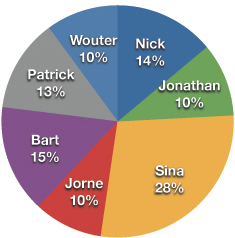
\includegraphics[height=6cm]{../../img/partition-1iter-1sem.jpg}
				\caption{Partition of working hours in iteration 1. \\ Period 12/10/09 - 04/01/10 (1st semester)}
				\label{fig:stats1-1}
				\end{center}
			\end{figure}
	
			Next, we analyze the statistics for the period February 08, 2010 - April 04, 2010. During this,
			everyone was encouraged to reach a specific target of working hours. This resulted in the statistics
			shown in table \ref{table:stats1-2}. \\
			
			\begin{table}
				\begin{center}
			\begin{tabular}{l c}
				\FL \textbf{Statistic} & \textbf{Result}
				\ML Number of weeks & 8
				\NN Total amount of hours  & 425
				\NN Average amount of hours/week & 53
			\end{tabular}
			\caption{General statistics for period 08/02/10 - 04/04/10.}
			\label{table:stats1-2}
			\end{center}
			\end{table}
			
			As we compare with table \ref{table:stats1-1}, we see that the weekly average remained more or less the same.
			However, figure \ref{fig:stats1-2} shows a substantial difference.  
			The re-organisation of responsibilities led to a drastically change in the partition of working hours. 
			This was obviously necessary in order to
			become a proportional working balance in the end. \\
			
			\begin{figure}
				\begin{center}
				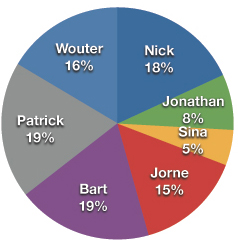
\includegraphics[height=6cm]{../../img/partition-1iter-2sem.jpg}
				\caption{Partition of working hours in iteration 1.\\ Period 08/02/10 - 04/04/10}
				\label{fig:stats1-2}
				\end{center}
			\end{figure}
			
			In general, we present the statistics for the complete first iteration in table \ref{table:stats1}. The 
			partition of working hours is prorated and well-balanced, taking into account the number of study-points. Every 
			team members worked more or less the same amount of time. This is 
			also shown by the pie chart
			in figure \ref{fig:stats1-3}.
			 
			\begin{table}
				\begin{center}
			\begin{tabular}{l c}
				\FL \textbf{Statistic} & \textbf{Result}
				\ML Number of weeks & 20
				\NN Total amount of hours  & 1050
				\NN Average amount of hours/week & 52.5
			\end{tabular}
			\caption{General statistics for iteration 1.}
			\label{table:stats1}
			\end{center}
			\end{table}
			
			\begin{figure}
				\begin{center}
				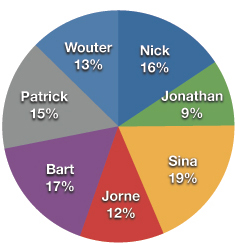
\includegraphics[height=6cm]{../../img/partition-1iter-total.jpg}
				\caption{Partition of working hours in iteration 1. \\ Period 12/10/09 - 04/04/10}
				\label{fig:stats1-3}
				\end{center}
			\end{figure}
			
			\subsection{Iteration 2}
			
			Iteration 2 started on April 05, 2010 and ended on May 23, 2010. It lasted only 7 weeks,
			which was much less than iteration 1 with 20 weeks. During this period, all documents were updated and some want-to-have requirements were implemented. Table \ref{table:stats2} gives the main statistics regarding this iteration. Note that the average amount of hours/week is lower than during the first iteration since multiple other projects required attention. A pie chart to denote the percentual partition of working hours in iteration 2 is given by figure \ref{fig:stats2}.
			
			\begin{table}
				\begin{center}
			\begin{tabular}{l c}
				\FL \textbf{Statistic} & \textbf{Result}
				\ML Number of weeks & 7
				\NN Total amount of hours  & 232
				\NN Average amount of hours/week & 33
			\end{tabular}
			\caption{General statistics for iteration 2: 05/04/10 - 23/05/10.}
			\label{table:stats2}
			\end{center}
			\end{table}
			
			\begin{figure}
				\begin{center}
				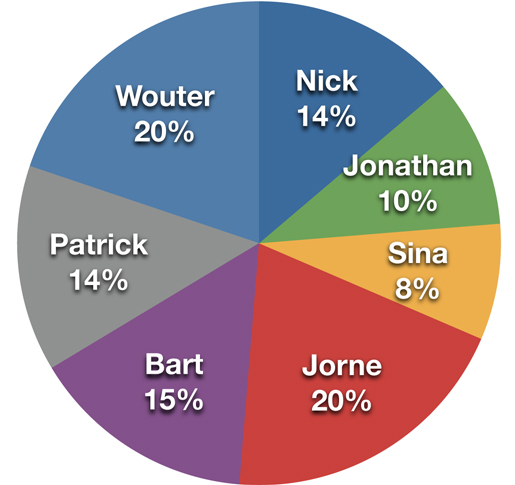
\includegraphics[height=6cm]{../../img/partition-2iter-total.jpg}
				\caption{Partition of working hours in iteration 2.}
				\label{fig:stats2}
				\end{center}
			\end{figure}
			
			\subsection{Total}
			
			When we put together the statistics presented in table \ref{table:stats1} and table \ref{table:stats2}, we obtain table \ref{table:stats3} which covers the period from October 12, 2009 - May 25, 2010, thus iteration 1 plus iteration 2.
			Moreover, figure \ref{fig:stats3} shows a pie chart to denote the percentual partition of working hours during this period. A summary of all timesheet statistics is given in Appendix \ref{appendix:statistics}.
			
			\begin{table}
				\begin{center}
			\begin{tabular}{l c}
				\FL \textbf{Statistic} & \textbf{Result}
				\ML Number of weeks & 27
				\NN Total amount of hours  & 1282
				\NN Average amount of hours/week & 47,5
			\end{tabular}
			\caption{General statistics for iteration 1 + 2.}
			\label{table:stats3}
			\end{center}
			\end{table}
			
			\begin{figure}
				\begin{center}
				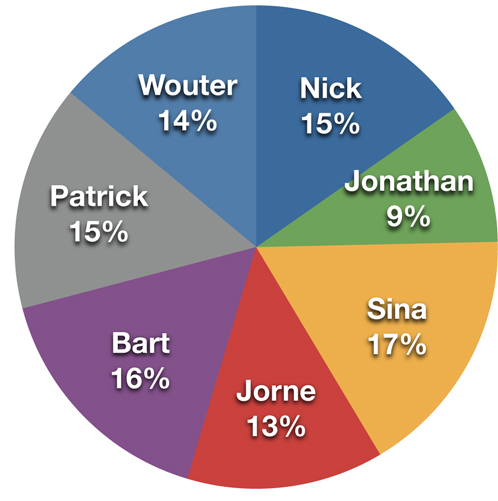
\includegraphics[height=6cm]{../../img/partition-total.jpg}
				\caption{Partition of working hours in iteration 1 + 2.}
				\label{fig:stats3}
				\end{center}
			\end{figure}
			
						
			
			\section{Costs}
			
			\subsection{Man-costs}
			\label{sec:costsofar}
			
			Using timesheets also enables to track the real cost of this project. Off course,
			this only includes man-costs and does not cover hidden problems that can occur during
			development. \\
			
			Considering the starter wage of a computer scientist is approximately \euro 2200 gross, we can calculate a 
			realistic earning per hour. Assume one should perform an average of 38 hours per week, 
			and a month consists of 4 weeks. This results in:
			\[ \textrm{Wage/hour} = \frac{\textrm{\euro} 2200 \textrm{ wage/month}}{38 \textrm{ hours/week} \cdot 4 \textrm{ weeks/month}} \approx \textrm{\euro} 14,50 \]
			 
			We know that the total amount of working hours, given in table \ref{table:stats1}, is 1050 hours. This 
			allows us to calculate the current man-cost:
			
			\[ \textrm{Total man-cost} = 1.282 \textrm{ working hours} \cdot 14,50 \textrm{ wage/hour} = \textrm{\euro} 18.589 \]
			
			
			
			\subsection{Estimation of total man-costs}
			
			During this project, we estimated the total cost
			based on the weekly average of working hours. Table \ref{table:estimations} shows all estimations made during the 27 weeks. It indicates that the weekly average of working hours is more or less consistent over time, which results in acceptable estimations compared with the final cost given in section \ref{sec:costsofar}. \\
			
			A cost is estimated with the following calculation:
			\[ \textrm{Estimated man-cost} =  \textrm{ working hours} \cdot 14,50 \textrm{ wage/hour} \cdot 27 \textrm{ weeks} = \textrm{\euro} 18.589 \]
			
			
			\begin{table}
				\begin{center}
			\begin{tabular}{l c c}
				\FL \textbf{Point in time} & \textbf{Weekly average} & \textbf{Estimated cost}
				\ML After 6 weeks & 47,16 h & \euro 17.936
				\NN Conference 1 & 55 h  & \euro 21.532
				\NN Conference 2 & 50 h & \euro 19.575
				\NN After iteration 1 & 52,5 h & \euro 20.590
			\end{tabular}
			\caption{All estimations of costs.}
			\label{table:estimations}
			\end{center}
			\end{table}
			
			\subsection{Estimation of effort}
			
			To calculate an estimation of costs, the COCOMO algorithm developed by Barry Boehm
			will be used. Depending on the number of lines of code, the costs and efforts of this
			project can be computed. Off course, this is just an estimation and will differ from
			reality. The algorithm provides next formulas in order to calculate the effort and
			cost:
			
			\begin{center}
			Effort Applied: $ E = a \cdot (KLOC)^{b} $ \\
			Development Time: $ D = c \cdot E^{d} $ \\
			People required: $ P = \frac{E}{D} $ \\
			\end{center}
			
			KLOC is the estimation of the code length expressed in thousands of lines of code.
			Our project can be classified as a semi-detached project which means that our team of
			a medium size has a mixed experience working with a mix of rigid and less than rigid
			requirements. Therefore, the parameters a, b, c, d are defined as in table \ref{par}. \\		
			
			
			\begin{table}
				\begin{center}
			\begin{tabular}{l l}
				\FL Parameter & Value
				\ML a & 3.0
				\NN b & 1.12
				\NN c & 2.5
				\NN d & 0.35
			\end{tabular}
				\end{center}
				\caption{COCOMO Parameters for a semi-detached project}
				\label{par}
			\end{table}	
			
			By analyzing simular projects, we estimate to write 10KLOC. This brings the total
			effort to:
			
			\begin{center}
				$ E = 3.0 \cdot 10^{1.12} \approx 39,55 $ man-months
			\end{center}
			
			The total development time thus becomes:
			
			\begin{center}
				$ D = 2,5 \cdot 39,55^{0,35} \approx 9,06 $ months
			\end{center}
			
			This results in a total staff estimation of
			
				\[ P = \frac{39,55 \textrm{ man-months}}{9,06 \textrm{ months}} \approx 4,37 \textrm{ people} \]
			
			Using the COCOMO algorithm, we can thus conclude that 4,37 people are needed to
			realise our project in 9,06 months. 
			
			\section {Dependencies}
			
			It was only possible to provide 1 general dependency :
			
			\begin{itemize}
				
				\item Iteration 2 depends on the completion of iteration 1.
				
			\end{itemize}
			
			
			\section{Planning}	
				\label{planning}
			\begin{figure}[h!]
				\begin{center}
				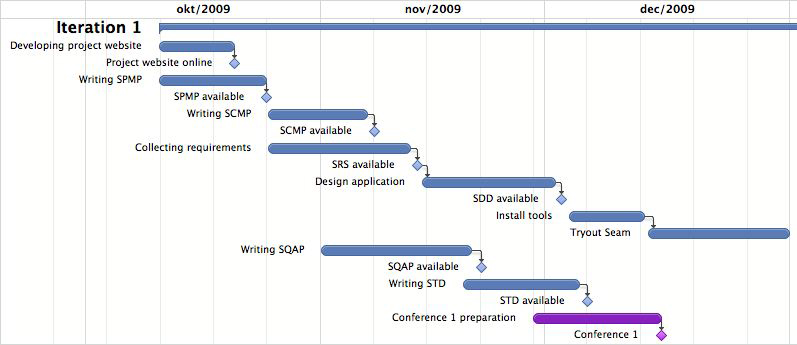
\includegraphics[angle=90, height=17cm]{../../img/gantt-chart-1iter-1.jpg}
				\caption{Planning iteration 1 in form of Gantt-chart - Part 1}
			\end{center}
			\end{figure}
			
				\begin{figure}
					\begin{center}
					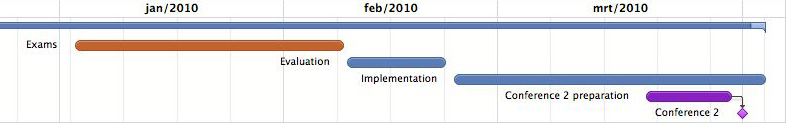
\includegraphics[angle=90, height=20cm]{../../img/gantt-chart-1iter-2.jpg}
					\caption{Planning iteration 1 in form of Gantt-chart - Part 2}
				\end{center}
				\end{figure}
			
				\begin{figure}
					\begin{center}
					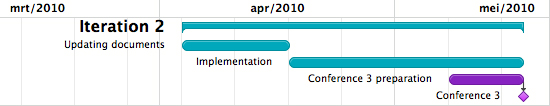
\includegraphics[angle=90, height=20cm]{../../img/gantt-chart-2iter.jpg}
					\caption{Planning iteration 2 in form of Gantt-chart}
				\end{center}
				\end{figure}
		

\appendix
\chapter{Timesheet Statistics}
\label{appendix:statistics}

\begin{figure}[h]
	\begin{center}
	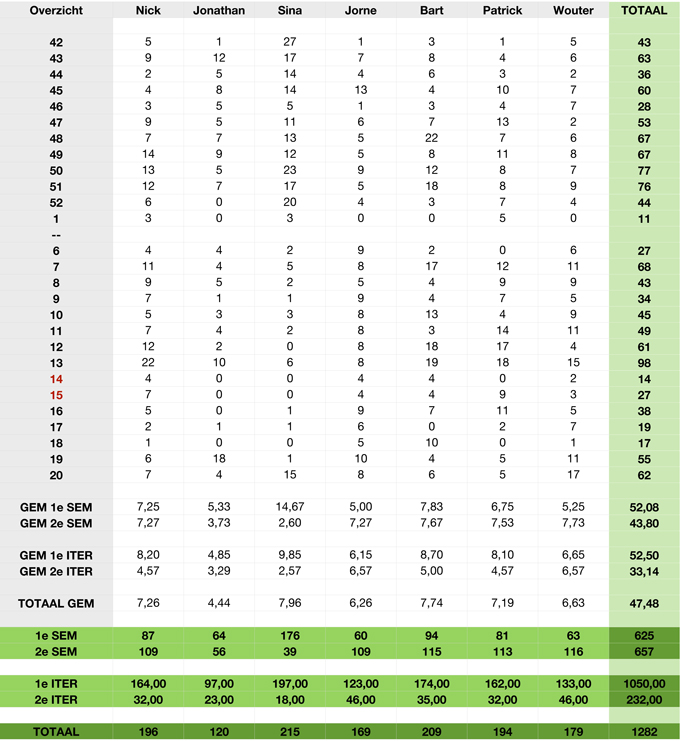
\includegraphics[width=13cm]{../../img/timesheet-table.jpg}
	\end{center}
\end{figure}

\begin{figure}[h]
	\begin{center}
	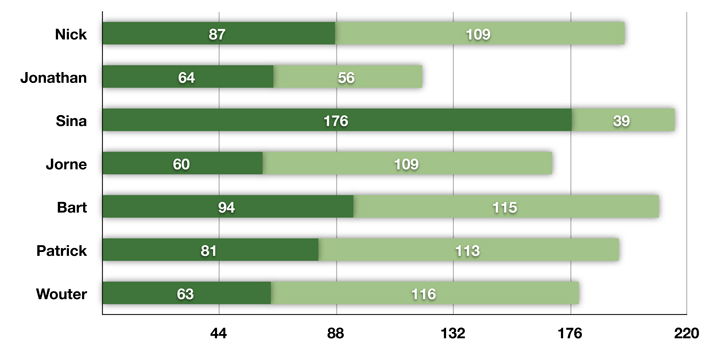
\includegraphics[width=15cm]{../../img/timesheet-bars.jpg}
	\end{center}
\end{figure}

\begin{figure}[h]
	\begin{center}
	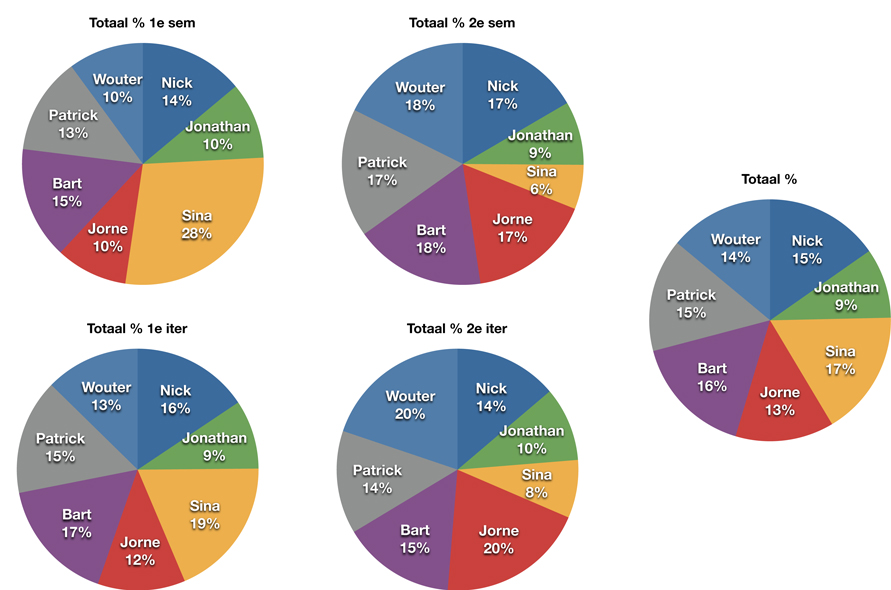
\includegraphics[width=15cm]{../../img/timesheet-pies.jpg}
	\end{center}
\end{figure} 


\renewcommand
{\bibname}
{\huge{Appendix B}\\
\vspace{12pt}
\Huge{References}}
\addcontentsline{toc}{chapter}{B References}
\setcounter{chapter}{1}

\begin{thebibliography}{9}
\bibitem{OOPerspective} Eric J. Braude, \emph{Software Engineering - An Object-Oriented Perspective}, John Wiley \& Sons, 2001. ISBN 0-471-32208-3.
\bibitem{slidesSE}
Dirk Vermeir \emph{\url{http://tinf2.vub.ac.be/~dvermeir/courses/software_engineering/slides.pdf}} 1 Nov 2009.
\end{thebibliography}



\end{projdoc}
\end{document}